%\documentclass{cumcmthesis}
\documentclass[withoutpreface,bwprint]{cumcmthesis} %去掉封面与编号页,电子版提交的时候使用。
\usepackage[superscript]{cite}
\usepackage{booktabs}
\usepackage{longtable}
\usepackage{float}
\usepackage{graphicx}
\usepackage{float}
\usepackage[framemethod=TikZ]{mdframed}
\usepackage{url}   % 网页链接
\usepackage{subcaption} % 子标题
\usepackage[linesnumbered,ruled,vlined]{algorithm2e} 
\usepackage{adjustbox}
\usepackage{algpseudocode}
\usepackage{longtable}


\title{基于...的电子产品生产决策模型}
 
\begin{document}
\maketitle
\begin{abstract}
	在企业生产电子产品的生产线中,需要考虑零配件供应商提供的零配件的次品率、生产个阶段中所产生的抽检及生产次品率、
	产品在出售之后的退换及拆解回收零配件等诸多问题。我们拟应用序贯概率比检测$SPRT$来作出抽样决策,并且综合生产
	次品的概率分布预测次品期望值,其后用$MGA$算法迭代找到最佳决策方案。最后建立了次品率波动曲线,再次迭代寻找的
	最优决策,增加了方案的可是配性。

	针对问题一,题目给出了两种情况,我们设计了基于$SPRT$的方法动态地作出抽样决策的方案,因为单次实验成功的期望服从二项分布,则利用
	标称值及扰动构建二项分布参数模型。依据题干中的情况我们假定了零假设和备择假设第i次取样的似然比,经过SPRT流程得到接受的假设。
	最后应用多层感知机$(MLP)$来拟合扰动函数得到最优表现的模型。经过假设检验,模型采样率小于3\%,且具备80\%以上的成功率,证实了策略的稳健性。

	针对问题二,题目已知平配件及成品的次品率,我们构建了单轮次决策向量,通过次品的概率分布能够计算出相应阶段的次品期望。为了能直观的
	体现决策方案对生产的影响,我们将多个生产轮次整合一个生产周期得到周期决策向量,由此列出不同决策下的净利润函数。通过$MGA$优化算法找到最优决策方案。

	针对问题三,本题与问题二一脉相承,增加了生产阶段和零配件的种类,与第二问类似构造单轮次决策向量并且整合为周期决策向量。在此基础上
	每轮零配件池及半成品池中的次品期望的要继承来自上一阶段的拆解零件,由此更新了产品净利润目标函数。最后通过遗传算法找到最优决策方案。

	针对问题四,我们对每个阶段次品率进行概率建模,并且运用高斯分布拟合之。考虑到采样期间会有各种偏出我们给标准高斯分布加入噪声
	已知次品率在工序流程中是可传播的,即可根据相邻工序的概率分布求的下个阶段的次品率。经过计算我们能够得到每个阶段次品率的标准差公式。
	带入问题二、三的模型中,我们能够得到更加符合实际的决策方案。

	\noindent{ \textbf{关键词:} Fisher精确检验\quad   多元线性回归\quad 系统聚类 \quad 灰色关联分析\quad}
\end{abstract}


\section{问题重述}
某电子产品的生产企业需要综合诸多考虑购置零部件、产品抽检、产品拆解、报废等问题,以确保产品质量的同时降低成本。

\textbf{问题一:}考虑到零配件供应商所述次品率不高于既定标称值,企业拟采用抽样检测方法以验收此批零配件。因为企业寻承担检测费用,企业希望应用数学模型得到最少抽检次数的抽样方案。

已知标称值为 10\%,结合以下两种不同情况,分别设计出具体的抽样检测方案:

1. 拒收条件:在95\%的置信水平下,如果检测结果表明零配件的次品率超出了标称值,那么这批零配件将被拒收。

2. 接收条件:在90\%的置信水平下,如果检测结果表明零配件的次品率未超过标称值,那么这批零配件将被接收。

\textbf{问题二:}在已知零配件及成品次品率情况下,在电子产品生产的零配件检测、装配、成品检测、不合格品拆解的各个阶段为企业作出最优决策。
并且结合判断依据及相应的指标对表1中企业在生产中遇到的情况作出相应的最优决策方案。

\textbf{问题三:}在零配件、半成品和成品的次品率已知情况下,重复问题2的生产决策方案以适配有m道工序、
n个零配件的问题。并且应用此方法针对表2中情况给出判断依据和指标得到最优的决策方案。

\textbf{问题四:}在零配件、半成品和成品的次品率均由抽样检测获得的情况下,重新考虑问题2、3的生产决策方案。
\section{问题分析}
\subsection{问题一的分析}
我们需要根据题目中给出的两种不同的情况,分别设计抽样检测方案。考虑单次检验为次品严格服从经典二项分布
,拟采用异常检测的经典取样方法:序贯概率比检测$SPRT$来动态地作出抽样决策。

\subsection{问题二的分析}
由于已知各零配件以及成品的次品率,依据排列组合我们能够得知在生产成品时零配件优劣的组合情况以及对应的概率分布。
又由于可能出现两个好的零部件组成一个坏的成品,综合成本考量我们是否需要考虑对成品进行拆解。
我们预先设置对零配件、成品的抽样检测及拆解参数(即:抽检(拆解)/不抽检(不拆解)),通过$MGA$算法多次模拟迭代实验得到最优的决策方案。
\subsection{问题三的分析}
问题三实际上是对问题二的一个延伸问题,增加了生产流程的阶段和零配件的数量,不过依然能够继承问题二中的思路。我们通过已知的平配件、半成品以及成品
的次品率对每一轮次生产多产生的次品情况分布进行考虑,计算出每个阶段的次品期望值。结合多轮次为一周期的决策向量及成本收益,我们运用优化算法
得到最优的决策方案。
\subsection{问题四的分析}
在问题四中我们需要根据抽样检测来确定,鉴于问题一中我们讨论的是单次检验的情况,我们能够构造零配件、半成品以及成品的次品率概率分布波动曲线。
将此处构造的次品率概率分布波动曲线代入问题二、三中的模型,求得更加符合实际的决策方案。
\section{基本假设与符号说明}
\subsection{基本假设}
$\bullet$ 假定每批零配件的次品率严格服从二项分布

$\bullet$ 假定每次抽检结果为次品的事件之间相互独立

$\bullet$ 假定每次生产的产品都能够流通到市场上(被客户购买)

\subsection{符号说明}
\begin{longtable}{m{3.5cm}<{\centering}m{10cm}<{\centering}}
	\toprule[1.5pt]
	\textbf{符号} & \textbf{含义}   \\ \midrule[1pt]
	\endfirsthead
	%
	\endhead
	%
	$N$         & 每批供应商提供的零配件总量 \\
	$D_{i}$     & 第$i$次抽检的零配件数量 \\
	$\mu$       & 次品率           \\
	$\nu$       & 产品中实际次品占比     \\
	$A$         & 拒真的决策边界       \\
	$B$         & 纳伪的决策边界       \\
	$LR$        & 似然比           \\
	$C$         & 决策向量          \\
	\bottomrule[1.5pt]
\end{longtable}

\section{问题一模型的建立与求解}
\subsection{问题一的模型建立}
针对每批零配件,假定总量为$N$,我们考虑采用异常检测的经典取样方法:序贯概率比检测$SPRT$作为抽检方案。在此之前
我们考虑每次取样的样本量为$D_i$,令单个零件次品与否的布尔值为$x$,考虑其单次试验成功(为次品)概率的期望为$\mu$,则其显然
服从经典的二项分布表示:
\begin{equation}
	\textit{Bern}(x|\mu) = \mu^x (1 - \mu)^{1-x}
\end{equation}
接下来考虑其在样本集上的对数似然函数,针对第$i$次取样$D_i$,对其中的每个样本取到观测$x_1,x_2...x_n$,根据题目要求
样本集中零配件的次品产生事件可认定为相互独立的。则其似然函数可写为:
\begin{equation}
	\mathbf{P}(D_i|\mu) = \prod_{n=1}^{N} p(x_n|\mu) = \prod_{n=1}^{N} \mu^{x_n} (1 - \mu)^{1-x_n}
\end{equation}
为便于后续处理,我们取其对数似然:
\begin{equation}
	\begin{split}
		&\ln\mathbf{P}(D|\mu) = \ln \prod_{n=1}^{N} \mu^{x_n} (1 - \mu)^{1-x_n}
		= \ln \mu \sum_{n=1}^{N} x_n + \ln(1 - \mu) \sum_{n=1}^{N} 1 - x_n \\
		&=  \ln \mu \sum_{n=1}^{N} x_n + \ln(1 - \mu) (N - \sum_{n=1}^{N} x_n)
		= \sum_{n=1}^{N} x_n \ln \mu + (1 - x_n) \ln(1 - \mu)
	\end{split}
\end{equation}
接下来我们依据题干给定零假设和备择假设:
\begin{equation}
	\begin{cases}
		H_0: \mu > 0.1 \\
		H_1: \mu \le 0.1
	\end{cases}
\end{equation}
题干中的两种情况意味着拒真和纳伪的显著性水平$\alpha$和$\beta$分别为0.05和0.1。在\textit{SPRT}语境下,考虑决策边界:
$$ A = \ln \frac{\beta}{1 - \alpha} \ \ \ \  B = \ln \frac{1 - \beta}{\alpha}$$
于是,针对每次采样$D_i$,我们需要求出在零假设和备择假设下的似然比$LR$:
\begin{equation}
	LR= \frac{\sum_{n=1}^{N} x_n \ln \mu_0 + (1 - x_n) \ln(1 - \mu_0)}{\sum_{n=1}^{N} x_n \ln \mu_1 + (1 - x_n) \ln(1 - \mu_1)}
\end{equation}
需要注意的是,在原生的$SPRT$场景中,$H_0$和$H_1$一般被认定为较为复杂的参数估计$\theta_0$和$\theta_1$,这取决于它们事先假定样本服从一个较为严谨且高度可表达的
概率分布。然而基于问题一,在没有明确历史数据和概率分布的先验情况下,我们只能将其建模为一般二项分布,
为了遵循$SPRT$的使用场景,我们将二项分布参数建模为$\mu_0=0.1+\Delta \mu_0$ , $\mu_1=0.1-\Delta \mu_1$。通过轻微扰动量来拟合样本的分布与所报标称值
的差异,扰动量的设置取决于样本量的大小,这点我们将在后续给出实验和说明。

尽管在许多场景中单样本取样策略以及被证明取得了很好的效果,但考虑到题干背景,我们依然选择样本集作为采样标准。遵循$SPRT$方法,给定总零配件量$N$,初次取样
$D_i$应为按照标称值所取的总样本配比,我们取$D_1=0.01N$,而后计算出当前样本下的对数似然比$LR_1$。序贯检验比方法遵循以下停止法则:
\begin{equation}
	\gamma = \inf \left\{ n | n \geq 1, LR_n \in (A, B) \right\}
\end{equation}
具体来说,若$LR_1 \le A$,接受$H_0$假设;若$LR_1 \ge B$,接受$H_1$假设,否则继续采样。初次采样的样本量为$D_1=0.01N$,假定每次
采样的次品数为$n_i$,则此后每次采样量依据以下法则确定:
\begin{equation}
	D_{i+1}=D_i-n_i
\end{equation}
\subsection{问题一的求解}
检验的完整流程可以作出如下表所示:

\begin{adjustbox}{width=16cm,height=6.5cm}
	\centering
	\begin{algorithm}[H]
		\SetAlgoLined
		\KwIn{总零配件数量 $N$,显著性水平 $\alpha$,第二类错误概率 $\beta$,扰动量 $\Delta \mu_0,\Delta \mu_1$}
		\KwOut{接受的假设 ($H_0$ 或 $H_1$)}
		计算决策边界 $A \gets \ln \frac{\beta}{1 - \alpha}$, $B \gets \ln \frac{1 - \beta}{\alpha}$\;
		设置 $\mu_0 \gets 0.1 + \Delta \mu_0$, $\mu_1 \gets 0.1 - \Delta \mu_1$\;
		初始样本量 $D_1 \gets 0.01N$n\;
		$i \gets 1$\;
		\While{TRUE}{
			取样 $D_i$ 个零配件,记录次品数量 $n_i$\;
			计算 $LR_i$:
			\[ LR_i = \frac{\sum_{n=1}^{D_i} x_n \ln \mu_0 + (1 - x_n) \ln(1 - \mu_0)}{\sum_{n=1}^{D_i} x_n \ln \mu_1 + (1 - x_n) \ln(1 - \mu_1)} \]
			\If{$LR_i \le A$}{
				接受零假设 $H_0$; \textbf{break}
			}
			\ElseIf{$LR_i \ge B$}{
				接受备择假设 $H_1$; \textbf{break}
			}
			\Else{
				$i \gets i+1$; $D_{i+1} \gets D_i - n_i$ \ \ 继续执行采样策略
			}
		}
		\Return 接受的假设 ($H_0$ 或 $H_1$)
		\label{alg:sprt}
		\caption{序贯概率比检验 (SPRT) 流程}
	\end{algorithm}
\end{adjustbox}

接下来我们考虑之前我们搁置的$\Delta \mu$的选取,这是该方案唯一的松弛参数;我们希望把它建模成一个函数而非定量。
这是由于我们面临一个相当大的搜索空间,它主要取决于两个因素:(1)总零配件数量$N$,由于该变量我们是不可控且无
先验的,所以我们暂且假定它的范围波动为$[1000,1000000]$;(2)真实标称值(Ground Truth) 我们也预先假定它的范围
波动为$[5\%,15\%]$。$\Delta \mu$的确定直接意味着SPRT策略的固定,面对庞大的搜索空间这样做显然是欠鲁棒的,因此寻找一种
对$\Delta \mu$的拟合$\Delta \mu = f(N,\theta)$是迫在眉睫的。其中N作为零配件总数是我们面临实际场景时的唯一自变量。$\theta$是拟合函数
的待优化参数。目标函数应该考虑到:(1)优化项:即尽可能减少取样量$D$;(2)惩罚项:即不出现误判的情况。于是它可以设计为:
\begin{equation}
	\Delta \mu = f(N,\theta) \ \ \ \ \ \ s.t. \ \underset{\theta}{\operatorname{argmax}} \ (\frac{1}{D} \times \mathbf{1}_H)
\end{equation}
这里的$\mathbf{1}_H$是对假设H的指示函数,用以表示最终选取的假设是否为真。
我们使用多层感知机(MLP)去拟合函数$f(N,\theta)$,自定虚拟数据集的范围遵循前文中给出的零件数量$N$和真实标称值的波动范围。
在1000个epoch中,我们选取测试集中精度最高的MLP模型作为评估基线以衡量SPRT的表现情况。最终结果如图\ref{Pro1_result}所示。
\begin{figure}[htbp]
	\centering
	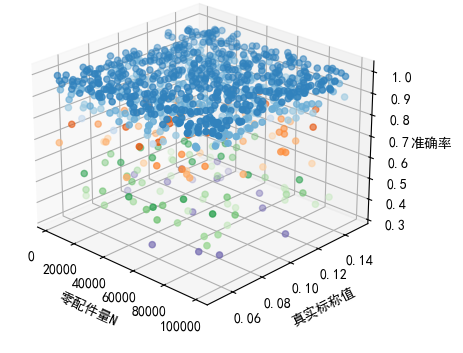
\includegraphics[width=0.48\textwidth]{Fig/Pro1_Accuracy.png}
	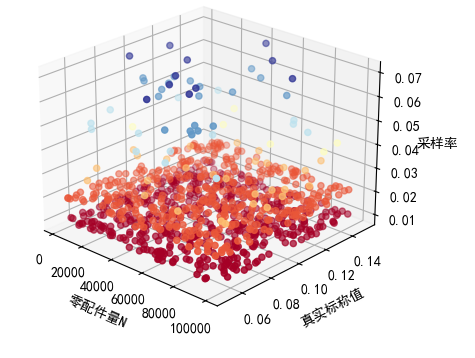
\includegraphics[width=0.48\textwidth]{Fig/Pro1_D.png}

	\begin{minipage}[b]{0.48\textwidth}
		\centering
		(a) 策略采样准确率
	\end{minipage}
	\begin{minipage}[b]{0.48\textwidth}
		\centering
		(b) 策略采样量占比
	\end{minipage}
	\caption{策略采样结果}
	\label{Pro1_result}
\end{figure}
具体来说,我们在$N$和真实标称值的预测范围内均匀采样;对于每个样本点,我们模拟100种样本集情况(这体现在零配件次品的分布次序上);在100种样本集中
由于$N$固定,我们拟合的$\Delta \mu$也固定,因此$SPRT$策略也是固定的,我们充分评估此基准上的假设判断成功率,发现在绝大多数情况下我们的策略都具备
80\%以上的成功率;由于总样本量的跨度较大,我们用策略共采集的样本量在总样本中的占比作为衡量指标,我们的采样占比绝大多数情况小于3\%,这充分体现了
我们采样策略的高效。此外根据我国工业检测国标:对于一般工业零件需要达到2\%-5\%的抽检率,对于高风险零件需要达到10\%以上的抽检率;我们的采样策略是
合乎标准且稳健的。
\section{问题二的模型建立与求解}
首先,我们可以将电子产品加工过程分为三个阶段,即:零配件、成品、市场。每当生产过程从一个阶段进入到另一个阶段均需要决策是否需要
进行抽检,将此过程抽象为图\ref{fig:pro2}。
\begin{figure}[H]
	\centering
	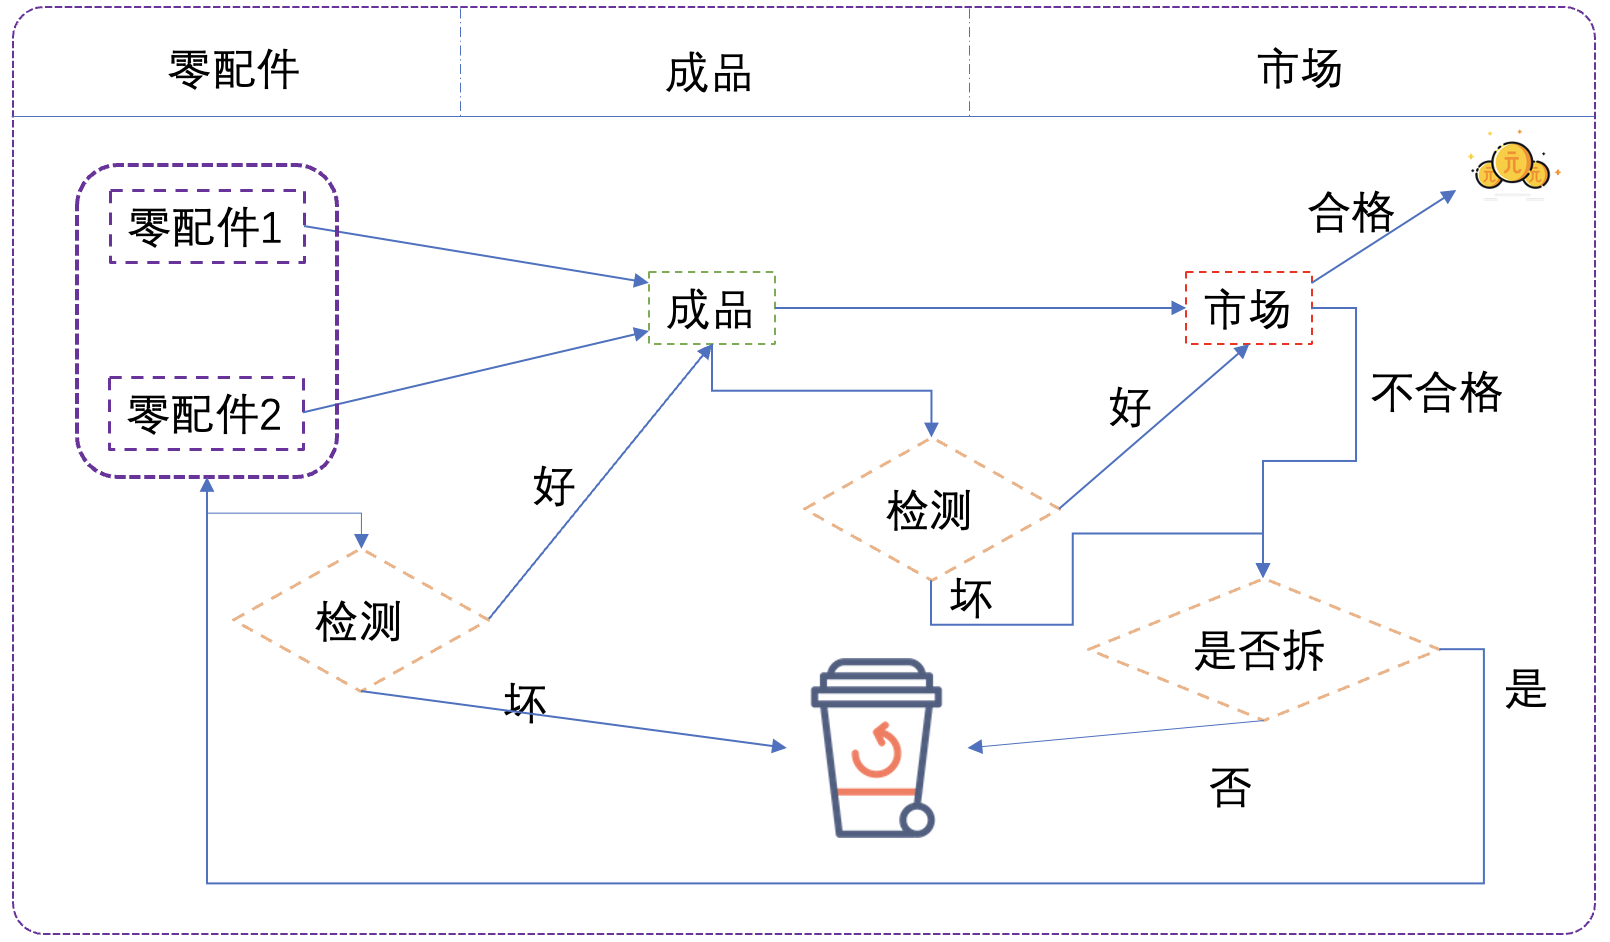
\includegraphics[width=0.8\textwidth,height = 0.4\textwidth]{Fig/pro2.png}      %获得的图片花括号中的名称为figure文件夹中重命名后的图片
	\caption{电子器件生产的流程图}
	\label{fig:pro2}
\end{figure}
\subsection{模型的建立}
在生产过程中我们设置一个列向量$\vec{C}=(c_{1},c_{2},c_{3},c_{4})^{T}$,其中的元素$c_i$分别表示
零配件1、零配件2、成品是否抽检及检测到不合格的成品是否拆解($c_{i}$的值为0时表示为不抽检/不拆解(丢弃),值为1时表示检测/拆解)。
我们的目标是通过合理的决策方案使得纯利润的期望值最最大。

因为零部件及成品的次品率已知,在每批零配件数目$N$足够大的情况下,我们可以通过对正次品进行排列组合,算出成品中的正次品零部件各种组合的概率。
在这里假设每批投入零部件1和零部件2的数目分别为$N_{1}$和$N_{2}$(这里的$N$足够大),其中$\mu_{1}$和$\mu_{2}$分别为零部件1、2的次品率,
则近似可以认为供应商提供的零部件1、2的次品数目为$N_{1}\cdot\mu_{1}$和$N_{2}\cdot\mu_{2}$。先考虑对零部件不进行检测直接拼装为成品并且成品不拆除的
情况$\vec{C}=(0,0,0,0)^{T}$,可以得出存在零部件次品的成品数目$k$的值域为$[\max \{N_{1}\cdot\mu_{1},N_{2}\cdot\mu_{2} \},N_{1}\cdot\mu_{1}+N_{2}\cdot\mu_{2}]$。
令$k$个成品中存在$i$和$j$个零配件1、2的次品个数。可以得到成品中有$i$个零配件1和$j$个零配件2的概率为$P_{i,j}$,计算公式如下:
\begin{equation}
	P_{i,j}=C_{N_{1}\cdot\mu_{1}}^{i}C_{N_{2}\cdot\mu_{2}}^{j}\mu_{1}^{i}\mu_{2}^{j}(1-\mu_{1})^{k-i}(1-\mu_{2})^{k-j}
	\label{eq:1}
\end{equation}
则$i$和$j$应当满足$i+j\ge k,i\le k,j\le k$,经过计算得到i和j的取值范围为$[k-j,k]$和$[\frac{k}{2},k]$。
我们假设$P_{k}$为存在次品零部件的成品数目为$k$的概率,计算公式如下:
\begin{equation}
	P_{k}=\sum_{i=k-j}^{k}\sum_{j=\frac{k}{2}}^{k}C_{N_{1}\cdot\mu_{1}}^{i}C_{N_{2}\cdot\mu_{2}}^{j}\mu_{1}^{i}\mu_{2}^{j}(1-\mu_{1})^{k-i}(1-\mu_{2})^{k-j}
	\label{eq:2}
\end{equation}
由此可以得到成品中的不合格产品的期望值$M$为($\mu_{3}$为成品次品率):
\begin{equation}
	M=\sum_{k=\max \{N_{1}\cdot\mu_{1},N_{2}\cdot\mu_{2} \}}^{N_{1}\cdot\mu_{1}+N_{2}\cdot\mu_{2}}k\cdot P_{k} + (\min \{ N1,N2\}-k)\cdot \mu_{3}\\
	\label{eq:3}
\end{equation}
令:产品售价为$p_{1}$检测零配件1、2及成品的费用分别为$f_{1}$、$f_{2}$和$f_{3}$,$f_{4}$和$f_{5}$为调换损失及拆解费用,则可以构造产生费用的行向量$\vec{F}=[N_{1}\cdot f_{1},N_{2}\cdot f_{2},\min \{N_{1},N_{2}\}\cdot f_{3},M\cdot f_{5}]$
,考虑产品在上一轮需要退换,我们设置$M^{-1}$为上一轮需要退换产品数(第一轮中$M^{-1}=0$)。的由此能够得到此轮次获利$Profit$:
\begin{equation}
	\textit{Profit}=(\min \{N_{1},N_{2}\}-M^{-1})\cdot p_{1}-\vec{F}\cdot \vec{C}-M\cdot f_{4}
	\label{eq:4}
\end{equation}
使函数适配16中不同的决策方案,我们需要定义每轮零配件池中所含数量$N'_{1}$、$N'_{2}$即包含每轮次固定补充数量$N_{1}$、$N_{2}$也包含上一轮次零产品拆解后补进的配件(即:$N'=N+M$)。
$M'$为新轮次中成品次品数目。则零配件池中为次品的平配件数目$n_{1}$、$n_{2}$的计算公式如下:
\begin{equation}
	n_{1}=N_{1}\cdot \mu_{1}+\sum_{j=\frac{k}{2}}^{k}\cdot P_{i,j} \qquad
	n_{2}=N_{2}\cdot \mu_{2}+\sum_{i=\frac{k}{2}}^{k}\cdot P_{i,j}
\end{equation}
在此基础上我们可以构造每轮次的收益$Profit$:
\begin{equation}
	\left\{\begin{matrix}
		\textit{Profit}=(\min \{N'_{1}-n_{1}\cdot c_{1},N'_{2}-n_{2}\cdot c_{2}\}-M')\cdot p_{1}-\vec{F}\cdot \vec{C}-M'\cdot f_{4} \\
		M'=[\sum_{k=\max \{n_{1},n_{2}\}}^{n_{1}+n_{2}}k\cdot P_{k} + (\min \{N'_{1}-n_{1}\cdot c_{1},N'_{2}-n_{2}\cdot c_{2}\}-k)\cdot \mu_{3}]\cdot c_{3}
	\end{matrix}\right.
	\label{eq:5}
\end{equation}
为了更直观的得到不同决策向量对电子产品生产的收益的影响,我们将图\ref{fig:pro2}中的单次生产流程抽象为一个生产轮次。在每个轮次中我们假设每轮
接受供应商提供的配件数目为固定的$N_{1}$、$N_{2}$,经过上一轮被检测为次品的零部件全部被舍弃,被拆解的成品中的零配件投入下一轮次的零配件池进入生产。
在每轮次生产中我们需要确定不同决策向量以保证电子产品生产的收益,于是我们拟定$t$个生产轮次为一个生产周期,每个生产周期中决策向量$\vec{C^{*}}=(c_{1},c_{2},\dots,c_{4t})^{T}$
为$t$个生产轮次中决策列向量$C$的叠加,如图\ref{fig:pro2-2}。
\begin{figure}[H]
	\centering
	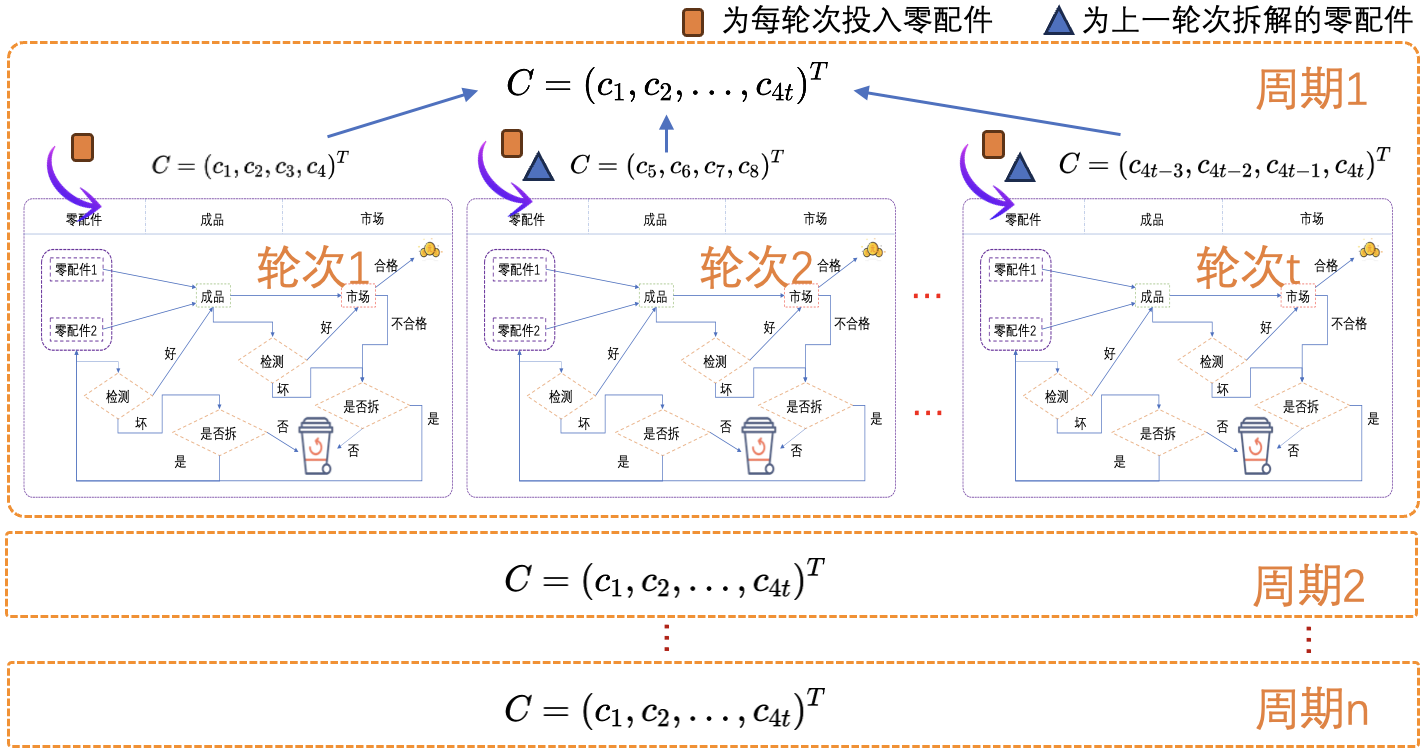
\includegraphics[width=0.8\textwidth]{Fig/pro2-2.png}
	\caption{产品决策周期图}
	\label{fig:pro2-2}
\end{figure}
综上我们构建了一个基于生产周期的决策模型,通过对每个生产周期中的决策向量$C^{*}$进行优化,就能够得到最优的决策方案。
$$	\max \quad  \textit{Profit}=\sum_{n=1}^{t}\left [  (\min \{N'_{1}-n_{1}\cdot c_{4n-3},N'_{2}-n_{2}\cdot c_{4n-2}\}-M')\cdot p_{1}-M'\cdot f_{4} \right ] -\vec{F}\cdot \vec{C^{*}}\\$$
\begin{equation*}
	s.t.\begin{cases}
		M'=[\sum_{k=\max \{n_{1},n_{2}\}}^{n_{1}+n_{2}}k\cdot P_{k}+(\min \{N'_{1}-n_{1}\cdot c_{4n-3},N'_{2}-n_{2}\cdot c_{4n-2}\}-k)\cdot \mu_{3}]\cdot c_{3}                                \\
		n_{1}=N_{1}\cdot \mu_{1}+\sum_{j=\frac{k}{2}}^{k}\cdot P_{i,j} \quad n_{2}=N_{2}\cdot \mu_{2}+\sum_{i=\frac{k}{2}}^{k}\cdot P_{i,j}                                                    \\
		N'_{1}=N_{1}+M \quad N'_{2}=N_{2}+M                                                                                                                                                    \\
		\vec{C^{*}}=(c_{1},c_{2},\dots,c_{4t})                                                                                                                                                 \\
		\vec{F^{*}}=[N_{1}\cdot f_{1},N_{2}\cdot f_{2},\min \{N_{1},N_{2}\}\cdot f_{3},M\cdot f_{5},N'_{1}\cdot f_{1},N'_{2}\cdot f_{2},\min \{N'_{1},N'_{2}\}\cdot f_{3},M'\cdot f_{5},\dots] \\
		P_{k}=\sum_{i=k-j}^{k}\sum_{j=\frac{k}{2}}^{k}C_{N_{1}\cdot\mu_{1}}^{i}C_{N_{2}\cdot\mu_{2}}^{j}\mu_{1}^{i}\mu_{2}^{j}(1-\mu_{1})^{k-i}(1-\mu_{2})^{k-j}                               \\
		P_{i,j}=C_{N_{1}\cdot\mu_{1}}^{i}C_{N_{2}\cdot\mu_{2}}^{j}\mu_{1}^{i}\mu_{2}^{j}(1-\mu_{1})^{k-i}(1-\mu_{2})^{k-j}
	\end{cases}
\end{equation*}
\subsection{模型的求解}
我们拟应用微生物遗传算法进行不断的迭代优化来寻找最优解,算法流程:

\begin{adjustbox}{width=16cm,height=6.5cm}
	\centering
	\begin{algorithm}[H]
		\SetAlgoLined
		\KwIn{每个段产生成本、检测成本、不合格品调换拆解费用和次品率$\mu$}
		\KwOut{单周期的成品收益$Profit$最优的决策向量$\vec{C^{*}}$}
		初始化一个周期为t轮次的决策列向量 $C^{*}$ 的种群,种群中的个体是随机生成的\;
		\While{TRUE}{
			从种群中随机选择两个个体 $\vec{C_{A}^{*}}$ 和 $\vec{C_{B}^{*}}$\;
			计算两个个体的$Profit$ \;
			\If{$ \textit{Profit}_{A} \le \textit{Profit}_{B}$}{
				winner $\gets \vec{C_{B}^{*}}$ \\
				loser $\gets \vec{C_{A}^{*}}$
			}
			\Else{
				winner $\gets \vec{C_{A}^{*}}$ \\
				loser $\gets \vec{C_{B}^{*}}$
			}
			\For{每个在loser的向量g}{
				\If{随机数 $r < \textit{crossoverRate}$}{
					随机选择winner中的一个向量h\;
					对g和h进行交叉操作\;
				}
			}
		}
		\Return 最优的决策向量$\vec{C^{*}}$
		\caption{微生物遗传算法 (MGA) 流程}
	\end{algorithm}
\end{adjustbox}
我们将周期设置为$1,2,3,\dots$轮次时发现每个周期的最佳决策向量$\vec{C^{*}}$中每轮次的决策向量趋近于一个定量值,
这意味着在同一情况下投入生产中无需变换决策向量来获得最大收益,在实际生产中也能够根据具体情况定期制定出一套检测、拆解标准方案。
结合问题中提供的6种不同情况我们得到以下决策方案:
\begin{longtable}{m{1.5cm}<{\centering}ccm{1.5cm}<{\centering}m{1.5cm}<{\centering}c}
	\caption{决策结果图}
    \label{tab:my-table}\\
	\hline
	情况 & 零配件1 & 零配件2 & 成品 & 拆解 & 最大纯利润(元/件) \\ \hline
	\endfirsthead
	%
	\endhead
	%
	\hline
	\endfoot
	%
	\endlastfoot
	%
	1  & 1    & 1    & 0  & 1  & 15.83 \\
	2  & 1    & 1    & 0  & 1  & 8.65  \\
	3  & 1    & 1    & 0  & 1  & 13.46 \\
	4  & 1    & 1    & 1  & 1  & 11.33 \\
	5  & 0    & 1    & 0  & 0  & 7.08  \\
	6  & 0    & 0    & 0  & 0  & 18.69 \\ \hline
	\end{longtable}
其中0代表不抽检/不拆解,1代表抽检/拆解。在不同的情况下,最大纯利润均有所不同,这是由于不同的情况下次品率、成本等不同,以至不同的最优决策方案。






\section{问题三的模型建立与求解}
首先沿用问题二的思路我们将生产加工过程分为四个阶段,即:零配件准备、半成品、成品、市场。每个阶段都需要决策出抽检方案,此过程可抽象为图\ref{fig:pro3-1}。
\begin{figure}[H]
	\centering
	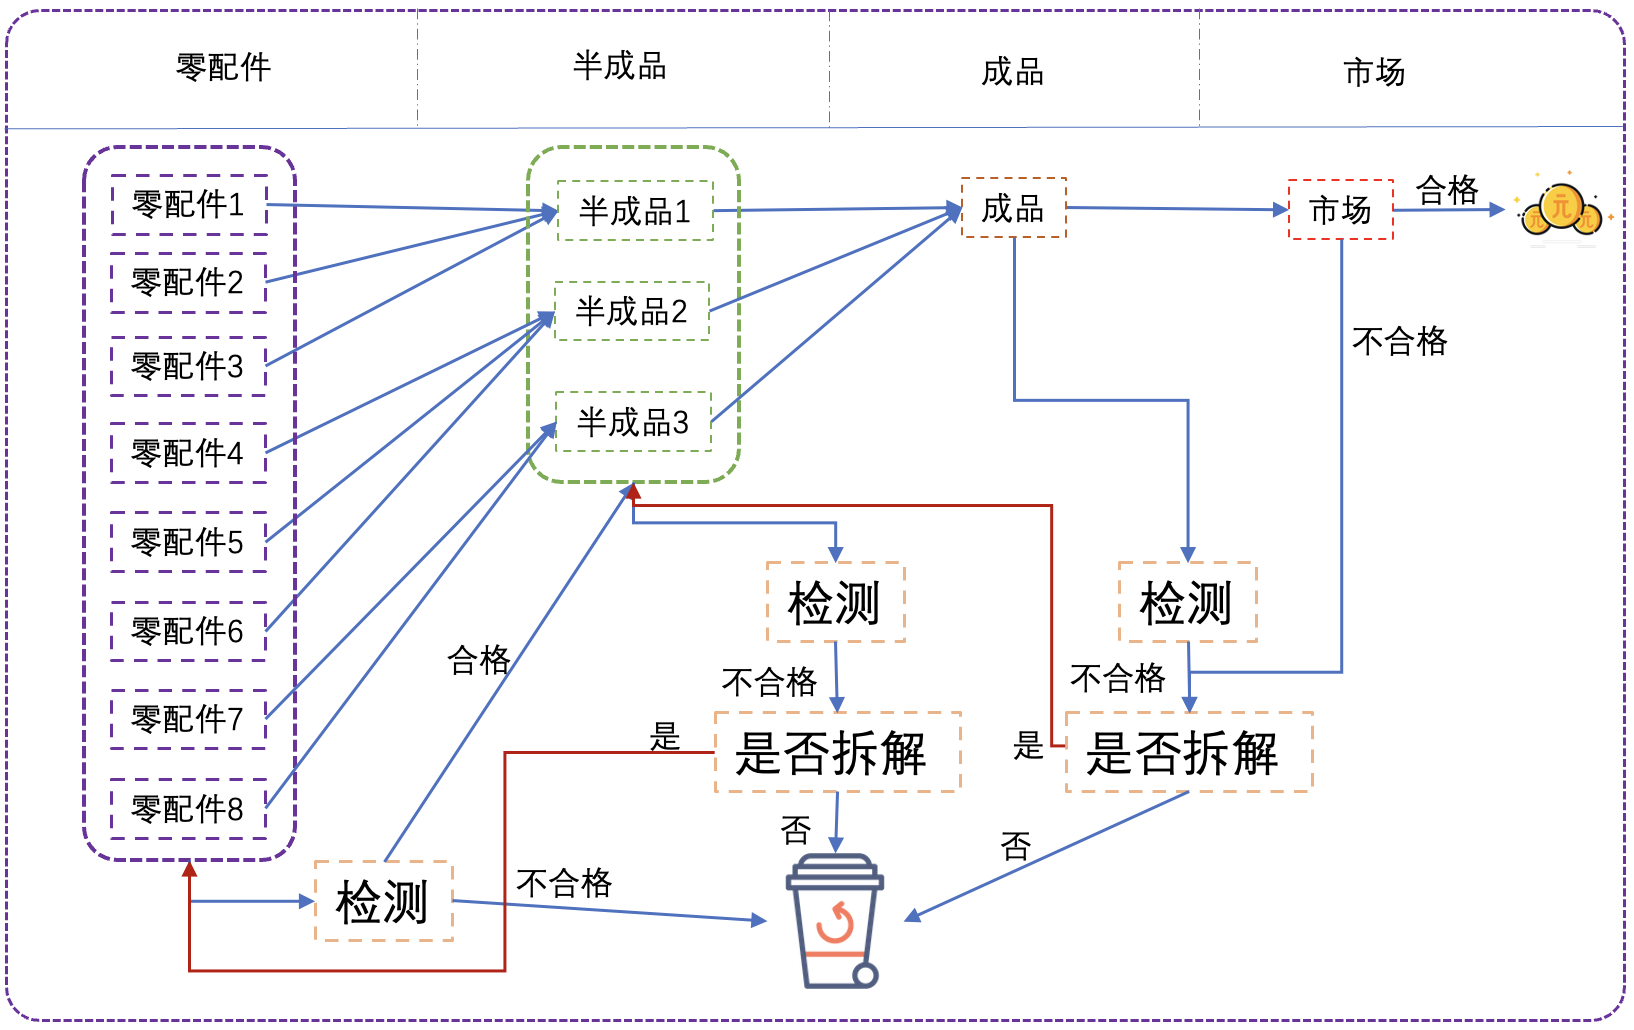
\includegraphics[width=0.8\textwidth]{Fig/pro3-1.png}
	\caption{电子器件生产四阶段的流程图}
	\label{fig:pro3-1}
\end{figure}
对于多个生产阶段的情况中我们设定所有的退货产品如果需要拆解则拆解为半成品,半成品拆解为零配件,然后将生产部件分别投入下一轮次的配件池和半成品池。
\subsection{模型的建立}
题目中要考虑推广到$m$道工序$n$个零配件的情况,我们可以将问题二的模型进行推广,构造决策向量为$\vec{C}=(c_{1},c_{2},\dots,c_{16})^{T}$,其中的元素$c_i$分别表示
零配件1$\sim$8、半成品1$\sim$3、成品是否抽检及检测到不合格的半成品、成品是否拆解($c_{i}$的值为0时表示为不抽检/不拆解(丢弃),值为1时表示检测/拆解)。
我们首先考虑对所有零配件、半成品、成品不进行检测不拆除的情况,即$\vec{C}=(0,0,\dots,0)^{T}$。这里假设半成品中存在次品零部件的半成品数目分别为$k_{1}$、$k_{2}$、$k_{3}$,
成品中存在次品零部件的成品数目为$k$。令8种零配件的次品率为$\mu_{1}$、$\mu_{2}$、$\dots$、$\mu_{8}$,半成品的次品率为$\mu'_{1}$、$\mu'_{2}$、$\mu'_{3}$,成品的次品率为$\mu''$。
与第二问相同我们假定每一轮次投入的零配件数是固定的数值$N_{1}$、$N_{2}$、$\dots$、$N_{8}$,则能够计算出零配件中存在次品的数目为$n_{1}$$\sim$$n_{8}$,其中$n_{i}=N_{i}\cdot\mu_{i}$
我么设置零配件池中的真实次品占比为$\nu_{1,1},\nu_{1,2},\dots,\nu_{1,8}$(在第一代时$\nu_{1,i}=\mu_{i}$)$\nu_{1,i}=\frac{M_{i}^{-1}+N_{i}\mu_{i}}{M_{i}^{-1}+N_{i}}$
这里我们用$M^{-1}$来表示上一轮退换回的产品数(第一轮里面$M^{-1}=0$)
以第一个半成品为例,可以得到存在次品零部件的半成品数目为$k_{1}$的概率$P_{k_{1}}$为:
\begin{equation}
	P_{k_{1}}=\sum_{i}\sum_{j}\sum_{z}C_{n_{1}}^{i}C_{n_{2}}^{j}C_{n_{3}}^{z}\nu_{1,1}^{i}\nu_{1,2}^{j}\nu_{1,3}^{z}(1-\nu_{1,1})^{k_{1}-i}(1-\nu_{1,2})^{k_{1}-j}(1-\nu_{1,3})^{k_{1}-z}
	\label{eq:6}
\end{equation}
其中$k_{1}$个半成品中存在的三个零配件情况为$i$、$j$、$z$,则需要满足$i+j+z \ge k_{1}$,$i\le k_{1}$,$j\le k_{1}$,$z\le k_{1}$。
由此能够算出半成品1中不合格品的期望值$M_{1}$为:
\begin{equation}
	M_{1}=\sum_{k_{1}=\max \{n_{1},n_{2},n_{3}\}}^{n_{1}+n_{2}+n_{3}}k_{1}\cdot P_{k_{1}}+(\min \{N_{1},N_{2},N_{3}\}-k_{1})\cdot \mu'_{1}
	\label{eq:7}
\end{equation}
同理可以得到半成品2、半成品3和成品的不合格品的期望值$M_{2}$、$M_{3}$:
\begin{align}
	M_{2}&=\sum_{k_{2}=\max \{n_{4},n_{5},n_{6}\}}^{n_{4}+n_{5}+n_{6}}k_{2}\cdot P_{k_{2}}+(\min \{N_{4},N_{5},N_{6}\}-k_{2})\cdot \mu'_{2} \\
	M_{3}&=\sum_{k_{3}=\max \{n_{7},n_{8}\}}^{n_{7}+n_{8}}k_{3}\cdot P_{k_{3}}+(\min \{N_{7},N_{8}\}-k_{3})\cdot \mu'_{3} 
	\label{eq:8}
\end{align}
接着我们能够通过不合格产品的期望算出各个半成品中存在次品的概率$\nu_{2,i}$为:
$$\nu_{2,i}=\frac{M_{i}^{-1}+\min \{ n_{1},n_{2},n_{3}\}}{M_{i}^{-1}+\min \{N_{1},N_{2},N_{3}\}}\qquad i=1,2,3$$
由此我们能够计算出成品中存在次品零部件的成品数目为$k$的概率$P_{k}$为:
\begin{equation}
	P_{k}=\sum_{i}\sum_{j}\sum_{z}C_{M_{1}}^{i}C_{M_{2}}^{j}C_{M_{3}}^{z}\nu_{2,1}^{i}\nu_{2,2}^{j}\nu_{2,3}^{z}(1-\nu_{2,1})^{k_{1}-i}(1-\nu_{2,2})^{k_{1}-j}(1-\nu_{2,3})^{k_{1}-z}
	\label{eq:9}
\end{equation}
其中$k$个成品中存在的三个次半成品情况为$i$、$j$、$z$,则需要满足$i+j+z \ge k$,$i\le k$,$j\le k$,$z\le k$。
由此能够算出成品中不合格品的期望值$M$为:
\begin{equation}
	M=\sum_{k=\max \{M_{1},M_{2},M_{3}\}}^{M_{1}+M_{2}+M_{3}}k\cdot P_{k}+(\min \{N_{1},N_{2},\dots,N_{8}\}-k)\cdot \mu''
	\label{eq:10}
\end{equation}
在理想情况下,多有的成品都进入市场,此时所产生的检测、退换、拆解费用为$\vec{F}=[N_{1}\cdot f_{1},N_{2}\cdot f_{2},\dots,N_{8}\cdot f_{8},
\min \{ N_{1},N_{2},N_{3}\}\cdot f_{9},\min \{ N_{4},N_{5},N_{6}\}\cdot f_{10},\min \{ N_{7},N_{8}\}\cdot f_{11},\\
\min \{N_{1},N_{2},\dots,N_{8}\}\cdot f_{12},M_{1}\cdot f_{13},M_{2}\cdot f_{14},M_{3}\cdot f_{15},M\cdot f_{16}]$,此行向量
中$f_{1}$$\sim$$f_{12}$均为抽样检测所产生的费用,$f_{13}$$\sim$$f_{16}$为次品拆解费用,$f_{16}$为退换产生费用。由此能够算出生产线检测、拆解、退换费$R$为:
\begin{equation}
	R=\vec{F}\cdot \vec{C} + M\cdot f_{17}
	\label{eq:11}
\end{equation}
综合考虑我们每轮需要调换上一轮里面次品的产品,而这一部分产品无法获利,这里我们用$M^{-1}$来表示上一轮退换回的产品数(第一轮里面$M^{-1}=0$),于是我们能够得到每轮次的收益$Profit$:
\begin{equation}
	\textit{Profit}=(\min \{N_{1},N_{2},\dots,N_{8}\}-M^{-1})\cdot p_{1}-R
	\label{eq:12}
\end{equation}
与问题二类似构建产品生产决策周期图,如图\ref{fig:pro3-2}。在这里我们将t个轮次的决策向量叠加到一起成为单周期决策向量$\vec{C}$。
随后,根据周期决策向量能够算出每一个周期的收益$Profit$,进过遗传进化算法能够找到最优的周期所含轮次$t$及最优的周期决策向量$\vec{C}$。
\begin{figure}[H]
	\centering
	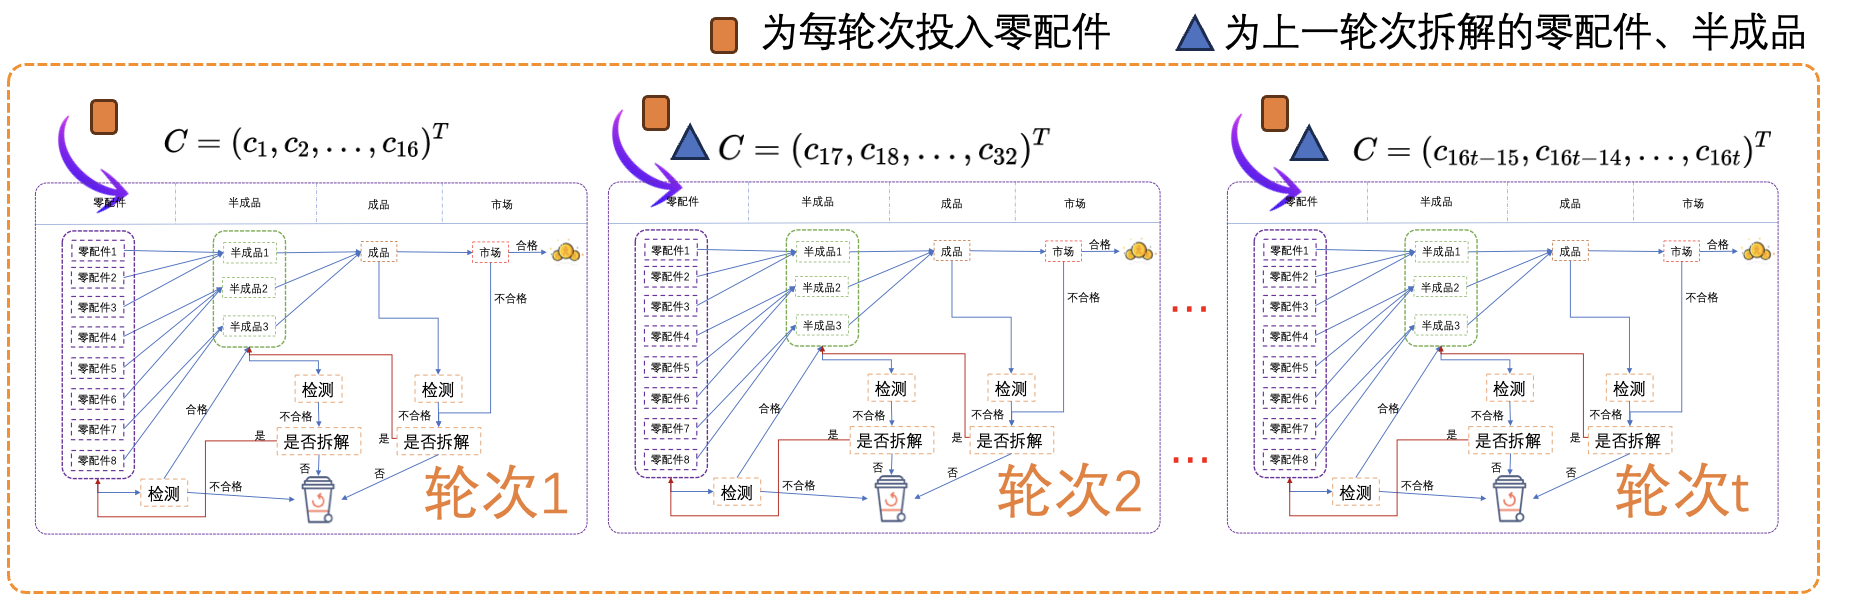
\includegraphics[width=0.8\textwidth]{Fig/pro3-2.png}
	\caption{产品决策周期图}
	\label{fig:pro3-2}
\end{figure}
综合上述算式,我们能够得到每轮次的收益$Profit$:
$$\max	\sum_{n=1}^{t}\textit{Profit}=(\min \{N_{1},N_{2},\dots,N_{8}\}-M_{(n)}^{-1})\cdot p_{1}-R$$
\begin{equation*}
s.t.\begin{cases}
	 R=\vec{F}\cdot \vec{C} + M\cdot f_{17}\\
	 M=\sum_{k=\max \{M_{1},M_{2},M_{3}\}}^{M_{1}+M_{2}+M_{3}}k\cdot P_{k}+(\min \{N_{1},N_{2},\dots,N_{8}\}-k)\cdot \mu''\\
	 M_{1}=\sum_{k_{1}=\max \{n_{1},n_{2},n_{3}\}}^{n_{1}+n_{2}+n_{3}}k_{1}\cdot P_{k_{1}}+(\min \{N_{1},N_{2},N_{3}\}-k_{1})\cdot \mu'_{1}\\
	 M_{2}=\sum_{k_{2}=\max \{n_{4},n_{5},n_{6}\}}^{n_{4}+n_{5}+n_{6}}k_{2}\cdot P_{k_{2}}+(\min \{N_{4},N_{5},N_{6}\}-k_{2})\cdot \mu'_{2}\\
	 M_{3}=\sum_{k_{3}=\max \{n_{7},n_{8}\}}^{n_{7}+n_{8}}k_{3}\cdot P_{k_{3}}+(\min \{N_{7},N_{8}\}-k_{3})\cdot \mu'_{3}\\
	 P_{k_{1}}=\sum_{i}\sum_{j}\sum_{z}C_{n_{1}}^{i}C_{n_{2}}^{j}C_{n_{3}}^{z}\nu_{1,1}^{i}\nu_{1,2}^{j}\nu_{1,3}^{z}(1-\nu_{1,1})^{k_{1}-i}(1-\nu_{1,2})^{k_{1}-j}(1-\nu_{
	 1,3})^{k_{1}-z}\\
	 P_{k_{2}}=\sum_{i}\sum_{j}\sum_{z}C_{n_{4}}^{i}C_{n_{5}}^{j}C_{n_{6}}^{z}\nu_{2,1}^{i}\nu_{2,2}^{j}\nu_{2,3}^{z}(1-\nu_{2,1})^{k_{2}-i}(1-\nu_{2,2})^{k_{2}-j}(1-\nu_{
	 2,3})^{k_{2}-z}\\
	 P_{k_{3}}=\sum_{i}\sum_{j}\sum_{z}C_{n_{7}}^{i}C_{n_{8}}^{j}\nu_{3,1}^{i}\nu_{3,2}^{j}(1-\nu_{3,1})^{k_{3}-i}(1-\nu_{3,2})^{k_{3}-j}\\
	 \nu_{1,i}=\frac{M_{i}^{-1}+N_{i}\mu_{i}}{M_{i}^{-1}+N_{i}} ,i=1,2,3\\
	\nu_{2,i}=\frac{M_{i}^{-1}+\min \{ n_{1},n_{2},n_{3}\}}{M_{i}^{-1}+\min \{N_{1},N_{2},N_{3}\}} i=1,2,3\\
	\end{cases}
\end{equation*}
\subsection{模型的求解}
与问题二中的求解方法类似,我们可以通过微生物遗传算法(MGA)进行不断遗传、竞争、重复、变异来寻找最优解,算法流程参见问题二中Algorithm 2中的描述。



\section{问题四的模型建立与求解}
\subsection{模型的建立}
本问题中我们需要考虑到抽样检测的准确性和应对风险的鲁棒性,而不能直接获取真实次品率:相比于对每个阶段的抽样进行风险建模,
一个更为直观的想法是对每一步的预测次品率$\mu$进行概率建模,这样做的好处是便于拟合我们在工序每阶段的概率分布(
这可以被看作是相互独立事件间的概率分布的传播)---我们选用
高斯分布拟合之。事实上,如果我们假定阶段p的期望为问题二及三中给定的次品率,那么:
\begin{equation}
	z_p = \mu_p + \sigma_p \odot \epsilon, \epsilon \sim \mathcal{N}(0, \mathbf{I})
\end{equation}
对于每次评估的$\mu_p$,我们只需计算出相应的风险参数$\sigma_p$,就可以重新从标准高斯分布中采样出噪声施加在其上:
\begin{equation}
	z \sim \mathcal{N}(z; \mu_p, \sigma_p^2 \mathbf{I})
\end{equation}
这样,实际的工序流程中次品率就被建模成了高斯分布,在优化过程中从中采样即可。接下来,我们论证该分布在工序流程中的可传播性。
事实上,如果我们把零配件的组装和成品看作一个马尔可夫过程,那么,概率分布的传播就可以视为一个前向动力学模型,针对任意的相邻两个工序(
我们暂且搁置对于一般的偏置项的考虑):
\begin{equation}
	\begin{split}
		P(z_{p+1} | z_p) &= \mathcal{N}(z_{p+1};z_p, \sigma_p^2 \mathbf{I}) \\
		&= \mu_{p+1}z_p + \sigma_{p+1} \odot \epsilon \\
		& = \mu_{p+1}(\mu_p + \sigma_p \odot \epsilon) + \sigma_{p+1} \odot \epsilon \\
		& = \mu_{p+1}\mu_p + (\mu_{p+1}\sigma_p + \sigma_{p+1} )\odot \epsilon
	\end{split}
\end{equation}
而又根据独立高斯分布的可加性:$\mathcal{N}(0, \sigma_1^2 \mathbf{I}) + \mathcal{N}(0, \sigma_2^2 \mathbf{I}) \sim \mathcal{N}(0, (\sigma_1^2 + \sigma_2^2) \mathbf{I})$
我们便可以得到$z_{p+1}$的分布:
\begin{equation}
	z_{p+1} \sim \mathcal{N}(z_{p+1}; \mu_{p+1}\mu_p, \sqrt{(\mu_{p+1}\sigma_p)^2 +\sigma_{p+1}^2}\mathbf{I})
\end{equation}
于是,我们的风险就可以通过前向动力学模型来传播了,$\mu$的期望依然遵循于预先设定的标准,而风险可以通过标准差逐层传递。

我们假设对问题二的零配件1,零配件2,成品;问题三的各种零配件,半成品,成品的次品率都采用$SPRT$进行抽样,我们预先设定$H_0$边界范围为:$[S_1,S_2]$;
取其初始值为$\frac{S_1+S_2}{2}$,每次确定其相对预设值的大小后,我们采用二分法逐渐收缩范围,重复10次,设定最终结果为$\mu_i$,并根据与样本集的真实误差
确定$\sigma_i$,在总样本中确定反复取得样本集,获得$\sigma_1,\sigma_2......\sigma_n$,考虑其拟合上文中的高斯分布:
\begin{equation}
	f(x; \sigma_p) = \frac{1}{\sigma_p \sqrt{2\pi}} \exp\left(-\frac{x^2}{2\sigma_p^2}\right)
\end{equation}
观测数据的似然函数是参数 $\sigma_p$ 的函数,它表示在给定参数 $\sigma_p$ 的情况下,观测到数据的概率。由于观测数据独立同分布,因此似然函数可以写成:
\begin{equation}
	L(\sigma_p) = \prod_{i=1}^n f(\sigma_i; \sigma_p) = \prod_{i=1}^n \frac{1}{\sigma_p \sqrt{2\pi}} \exp\left(-\frac{\sigma_i^2}{2\sigma_p^2}\right)
\end{equation}
取其对数似然:
\begin{equation}
	\begin{split}
		\ln L(\sigma_p) &= \sum_{i=1}^n \ln(f(\sigma_i; \sigma_p)) = \sum_{i=1}^n \left[ \ln\left(\frac{1}{\sigma_p \sqrt{2\pi}}\right) - \frac{\sigma_i^2}{2\sigma_p^2} \right] \\
		&= -n \ln(\sigma_p) - n \ln(\sqrt{2\pi}) - \frac{1}{2\sigma_p^2} \sum_{i=1}^n \sigma_i^2
	\end{split}
\end{equation}
求解上述方程,得到参数 $\sigma_p$ 的 MLE 估计值:
\begin{equation}
	\hat{\sigma}_p = \sqrt{\frac{\sum_{i=1}^n \sigma_i^2}{n}}
\end{equation}
\subsection{模型的求解}
根据上述的次品率的模型能够算出每个阶段产品的标称值,由此我们给原本各阶段的次品率加上标准差的估计值。
因为标准差的估计是分阶段判断的,现在拟将零配件阶段的,半成品阶段和成品阶段的标准差定位为$\sigma_{1}$,$\sigma_{2}$,$\sigma_{3}$。
则第二问可以将决策方案的目标函数及约束条件改为:
$$	\max \quad  \textit{Profit}=\sum_{n=1}^{t}\left [  (\min \{N'_{1}-n_{1}\cdot c_{4n-3},N'_{2}-n_{2}\cdot c_{4n-2}\}-M')\cdot p_{1}-M'\cdot f_{4} \right ] -\vec{F}\cdot \vec{C^{*}}\\$$
\begin{equation*}
	s.t.\begin{cases}
		M'=[\sum_{k=\max \{n_{1},n_{2}\}}^{n_{1}+n_{2}}k\cdot P_{k}+(\min \{N'_{1}-n_{1}\cdot c_{4n-3},N'_{2}-n_{2}\cdot c_{4n-2}\}-k)\cdot (\mu_{3}+\sigma_{3}\varepsilon )]\cdot c_{3}                                \\
		n_{1}=N_{1}\cdot (\mu_{1}+\sigma_{1}\varepsilon )+\sum_{j=\frac{k}{2}}^{k}\cdot P_{i,j} \quad n_{2}=N_{2}\cdot (\mu_{2}+\sigma_{2}\varepsilon )+\sum_{i=\frac{k}{2}}^{k}\cdot P_{i,j}                                                    \\
		N'_{1}=N_{1}+M \quad N'_{2}=N_{2}+M                                                                                                                                                    \\
		\vec{C^{*}}=(c_{1},c_{2},\dots,c_{4t})                                                                                                                                                 \\
		\vec{F^{*}}=[N_{1}\cdot f_{1},N_{2}\cdot f_{2},\min \{N_{1},N_{2}\}\cdot f_{3},M\cdot f_{5},N'_{1}\cdot f_{1},N'_{2}\cdot f_{2},\min \{N'_{1},N'_{2}\}\cdot f_{3},M'\cdot f_{5},\dots] \\
		P_{k}=\sum_{i=k-j}^{k}\sum_{j=\frac{k}{2}}^{k}C_{N_{1}\cdot\mu_{1}}^{i}C_{N_{2}\cdot\mu_{2}}^{j}(\mu_{1}+\sigma_{1}\varepsilon)^{i}(\mu_{2}+\sigma_{2}\varepsilon)^{j}(1-\mu_{1}+\sigma_{1}\varepsilon)^{k-i}(1-\mu_{2}+\sigma_{2}\varepsilon)^{k-j}                               \\
		P_{i,j}=C_{N_{1}\cdot\mu_{1}}^{i}C_{N_{2}\cdot\mu_{2}}^{j}(\mu_{1}+\sigma_{1}\varepsilon)^{i}(\mu_{2}+\sigma_{2}\varepsilon)^{j}(1-\mu_{1}+\sigma_{1}\varepsilon)^{k-i}(1-\mu_{2}+\sigma_{2}\varepsilon)^{k-j}   
	\end{cases}
\end{equation*}
同理在第三问中,我们可以将决策方案的目标函数及约束条件改为:
$$\max	\sum_{n=1}^{t}\textit{Profit}=(\min \{N_{1},N_{2},\dots,N_{8}\}-M_{(n)}^{-1})\cdot p_{1}-R$$
\begin{equation*}
s.t.\begin{cases}
	 R=\vec{F}\cdot \vec{C} + M\cdot f_{17}\\
	 M=\sum_{k=\max \{M_{1},M_{2},M_{3}\}}^{M_{1}+M_{2}+M_{3}}k\cdot P_{k}+(\min \{N_{1},N_{2},\dots,N_{8}\}-k)\cdot \mu''\\
	 M_{1}=\sum_{k_{1}=\max \{n_{1},n_{2},n_{3}\}}^{n_{1}+n_{2}+n_{3}}k_{1}\cdot P_{k_{1}}+(\min \{N_{1},N_{2},N_{3}\}-k_{1})\cdot \mu'_{1}\\
	 M_{2}=\sum_{k_{2}=\max \{n_{4},n_{5},n_{6}\}}^{n_{4}+n_{5}+n_{6}}k_{2}\cdot P_{k_{2}}+(\min \{N_{4},N_{5},N_{6}\}-k_{2})\cdot \mu'_{2}\\
	 M_{3}=\sum_{k_{3}=\max \{n_{7},n_{8}\}}^{n_{7}+n_{8}}k_{3}\cdot P_{k_{3}}+(\min \{N_{7},N_{8}\}-k_{3})\cdot \mu'_{3}\\
	 P_{k_{1}}=\sum_{i}\sum_{j}\sum_{z}C_{n_{1}}^{i}C_{n_{2}}^{j}C_{n_{3}}^{z}\nu_{1,1}^{i}\nu_{1,2}^{j}\nu_{1,3}^{z}(1-\nu_{1,1})^{k_{1}-i}(1-\nu_{1,2})^{k_{1}-j}(1-\nu_{
	 1,3})^{k_{1}-z}\\
	 P_{k_{2}}=\sum_{i}\sum_{j}\sum_{z}C_{n_{4}}^{i}C_{n_{5}}^{j}C_{n_{6}}^{z}\nu_{2,1}^{i}\nu_{2,2}^{j}\nu_{2,3}^{z}(1-\nu_{2,1})^{k_{2}-i}(1-\nu_{2,2})^{k_{2}-j}(1-\nu_{
	 2,3})^{k_{2}-z}\\
	 P_{k_{3}}=\sum_{i}\sum_{j}\sum_{z}C_{n_{7}}^{i}C_{n_{8}}^{j}\nu_{3,1}^{i}\nu_{3,2}^{j}(1-\nu_{3,1})^{k_{3}-i}(1-\nu_{3,2})^{k_{3}-j}\\
	 \nu_{1,i}=\frac{M_{i}^{-1}+N_{i}(\mu_{i}+\sigma_{i})}{M_{i}^{-1}+N_{i}} ,i=1,2,3\\
	\nu_{2,i}=\frac{M_{i}^{-1}+\min \{ n_{1},n_{2},n_{3}\}}{M_{i}^{-1}+\min \{N_{1},N_{2},N_{3}\}} i=1,2,3\\
	\end{cases}
\end{equation*}
经过求解可以得到最优的决策向量$\vec{C}$
\section{灵敏度分析}
\section{模型评价}

%参考文献
\begin{thebibliography}{9}%宽度9
    \bibitem[1]{luojiawei2019latex}
    
    \bibitem[2]{}

    \bibitem[3]{}
    
    \bibitem[4]{}
   
    \bibitem[5]{}
   
    \bibitem[6]{}
   
    \bibitem[7]{}
   
    \bibitem[8]{}
   
\end{thebibliography}

\newpage
%附录
\begin{appendices}
	\section{代码2}
	 
	\begin{lstlisting}[language=matlab]
	kk=2;[mdd,ndd]=size(dd);
	 
	 \end{lstlisting}
	 
	 \section{代码2}
	 
	\begin{lstlisting}[language=c]
	kk=2;
	[mdd,ndd]=size(dd);
	 \end{lstlisting}
	\end{appendices}
\end{document}
